\documentclass[../main.tex]{subfiles}

\begin{document}
\section{درباره جنگ ستارگان}

\subsection{مقدمه}
\paragraph{}
همانطور که در طول درس هم متوجه شده‌اید، پرهام مجموعه فیلم‌های جنگ ستارگان\LTRfootnote{The Star Wars} را دوست دارد.
در این سوال قصد داریم یک وب‌سایت ساده برای جمع‌آوری اطلاعات این مجموعه فیلم طراحی کنیم.

\subsection{وب‌سایت}
\paragraph{}
این وب‌سایت از شمای زیر پیروی می‌کند. در این شما یک عکس پس‌زمینه وجود داشته و محتوا در قالب یک مستطیل با پس‌زمینه شفاف روی آن نمایش داده می‌شود.
در نظر داشته باشید که عکس پس‌زمینه می‌بایست تمام صفحه را پوشانده باشد و در صورتی که از صفحه بزرگتر باشد \textbf{نباید} باعث ایجاد \lr{scrollbar} گردد.
در شرایطی که ابعاد صفحه نمایش مناسب نباشد می‌بایست عکس در وسط زوم شود.

\begin{figure}[h]
  \centering
  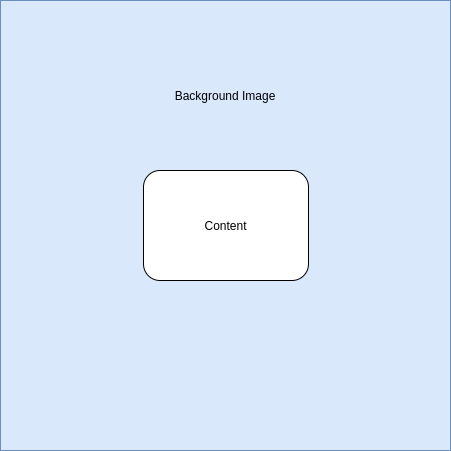
\includegraphics[scale=0.25]{./swapi-top-level}
  \caption{طراحی سطح بالا}
\end{figure}

\paragraph{}
مستطیل میانی تمامی محتویات قابل نمایش شما را می‌بایست شامل شود. این مستطیل می‌بایست تنها به اندازه محتویات باشد اما برای نمایش زیباتر برای آن \lr{padding} در نظر بگیرید.
محتوای مورد نمایش شما، ۱۰ مورد اول از کشتی‌فضایی\LTRfootnote{Starship}‌های مجموعه جنگ‌ستارگان برگرفته از تارنمای زیر می‌باشد:

\begin{latin}
  \url{https://swapi.dev/}
\end{latin}

توجه داشته باشید که در اینجا لزوما تمام شناسه‌ها موجود نمی‌باشند بنابراین ۱۰ کشتی‌فضایی اول لزوما شناسه‌ی ۱ تا ۱۰ نخواهند داشت.

\Extra پیاده‌سازی صفحه‌گذاری\LTRfootnote{pagination}

\begin{figure}[h]
  \centering
  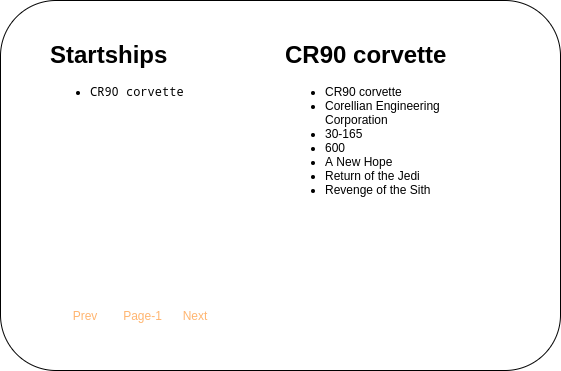
\includegraphics[scale=0.25]{./swapi-content}
  \caption{طراحی مستطیل محتوا}
\end{figure}

\paragraph{}
کاربر می‌تواند از لیست این کشتی‌فضایی‌ها یکی را انتخاب کرده و جزئیات آن را ببیند. اگر بخواهیم دقیقتر صحبت کنیم لیست شامل \textit{نام} ۱۰ کشتی‌فضایی است که با کلیک بر روی هر یک اطلاعات جزئی آن شامل \textit{مدل}، \textit{سازنده}، \textit{خدمه} و \textit{تعداد مسافران} نمایان می‌گردد.
برای نمونه داده‌ای که شما برای یک کشتی فضایی دریافت می‌کنید در ادامه آورده شده است.

\begin{latin}
\begin{lstlisting}[]
{
    "name": "Imperial shuttle",
    "model": "Lambda-class T-4a shuttle",
    "manufacturer": "Sienar Fleet Systems",
    "cost_in_credits": "240000",
    "length": "20",
    "max_atmosphering_speed": "850",
    "crew": "6",
    "passengers": "20",
    "cargo_capacity": "80000",
    "consumables": "2 months",
    "hyperdrive_rating": "1.0",
    "MGLT": "50",
    "starship_class": "Armed government transport",
    "pilots": [
        "http://swapi.dev/api/people/1/",
        "http://swapi.dev/api/people/13/",
        "http://swapi.dev/api/people/14/"
    ],
    "films": [
        "http://swapi.dev/api/films/2/",
        "http://swapi.dev/api/films/3/"
    ],
    "created": "2014-12-15T13:04:47.235000Z",
    "edited": "2014-12-20T21:23:49.900000Z",
    "url": "http://swapi.dev/api/starships/22/"
}
\end{lstlisting}
\end{latin}

در صورتی که قسمت فیلم‌ها نیز دارای اطلاعات باشد می‌بایست نام فیلم‌ها ذکر شود. دقت کنید برای این امر نیاز به یک تقاضای جداگانه برای فیلم دارید. ساختار \lr{URL}ها در اینجا بسیار ساده می‌باشند ولی در جهت تاکید در قسمت زیر آن‌ها را مرور کرده‌ایم:

\begin{itemize}\begin{latinitems}
  \item https://swapi.dev/api/starships/<id>
  \item https://swapi.dev/api/films/<id>
\end{latinitems}\end{itemize}


\subsection{نکات پیاده‌سازی}

\begin{itemize}
    \item آنچه در شما آورده شده است برای فهم بهتر شما می‌باشد بنابراین سعی کنید تا حد امکان وب‌سایت را گویا طراحی کنید.
    \item برای کدهایتان از کامنت استفاده کنید. توضیح کارکرد بلاک‌های \lr{css} اجباری می‌باشد. توابعی و قطعات کد جاوا اسکریپت نیز می‌بایست حداقل یک خط کامنت داشته باشند.
    \item کامنت فارسی یا انگلیسی موردی ندارد اما از فینگلیش (!) نوشتن پرهیز کنید.
    \item استفاده از کتابخانه‌ها و فریم‌ورک‌ها در پروژه مجاز \textbf{نمی‌باشد}.
    \item از آنجایی که این پروژه در قالب \textbf{امتحان میانترم} می‌باشد از تغییر دادن صورت مساله یا انجام موارد خارج از موارد مطرح شده خودداری کنید.
\end{itemize}

\end{document}
